% Template for PLoS
% Version 3.1 February 2015

\documentclass[10pt,letterpaper]{article}
\usepackage[top=0.85in,left=2.75in,footskip=0.75in]{geometry}

% Use adjustwidth environment to exceed column width (see example table in text)
\usepackage{changepage}

% Use Unicode characters when possible
\usepackage[utf8]{inputenc}

% textcomp package and marvosym package for additional characters
\usepackage{textcomp,marvosym}

% fixltx2e package for \textsubscript
\usepackage{fixltx2e}

% amsmath and amssymb packages, useful for mathematical formulas and symbols
\usepackage{amsmath,amssymb}

% cite package, to clean up citations in the main text. Do not remove.
\usepackage{cite}

% Use nameref to cite supporting information files (see Supporting Information section for more info)
\usepackage{nameref,hyperref}

% line numbers
\usepackage[right]{lineno}

% ligatures disabled
\usepackage{microtype}
\DisableLigatures[f]{encoding = *, family = * }

% rotating package for sideways tables
\usepackage{rotating}

% Remove comment for double spacing
%\usepackage{setspace} 
%\doublespacing

% Text layout
\raggedright
\setlength{\parindent}{0.5cm}
\textwidth 5.25in 
\textheight 8.75in

% Bold the 'Figure #' in the caption and separate it from the title/caption with a period
% Captions will be left justified
\usepackage[aboveskip=1pt,labelfont=bf,labelsep=period,justification=raggedright,singlelinecheck=off]{caption}

% Use the PLoS provided BiBTeX style
\bibliographystyle{plos2015}

% Remove brackets from numbering in List of References
\makeatletter
\renewcommand{\@biblabel}[1]{\quad#1.}
\makeatother

% Leave date blank
\date{}

% Header and Footer with logo
\usepackage{lastpage,fancyhdr,graphicx}
\usepackage{epstopdf}
\pagestyle{myheadings}
\pagestyle{fancy}
\fancyhf{}
\lhead{
\includegraphics[width=2.0in]{PLOS-submission.eps}}
\rfoot{\thepage/\pageref{LastPage}}
\renewcommand{\footrule}{\hrule height 2pt \vspace{2mm}}
\fancyheadoffset[L]{2.25in}
\fancyfootoffset[L]{2.25in}
\lfoot{\sf PLOS}

%% Include all macros below

\newcommand{\lorem}{{\bf LOREM}}
\newcommand{\ipsum}{{\bf IPSUM}}

%% END MACROS SECTION


\begin{document}
\vspace*{0.35in}

% Title must be 250 characters or less.
% Please capitalize all terms in the title except conjunctions, prepositions, and articles.
\begin{flushleft}
{\Large
\textbf\newline{Ten Simple Rules for Taking Advantage of GitHub in Bioinformatics}
}
\newline
\\
Yasset Perez-Riverol\textsuperscript{1,*},
Rui Wang\textsuperscript{1},
Timo Sachsenberg\textsuperscript{2},
Julian Uszkoreit\textsuperscript{3},
Laurent Gatto\textsuperscript{4},
Felipe da Veiga Leprevost\textsuperscript{5},
Christian Fufezan\textsuperscript{6},
Juan Antonio Vizcaíno\textsuperscript{1,*}

\bigskip

\bf{1} European Molecular Biology Laboratory, European Bioinformatics
Institute (EMBL-EBI), Wellcome Trust Genome Campus, Hinxton,
Cambridge, CB10 1SD, UK.
\\
\bf{2} Applied Bioinformatics and Department of Computer Science,
University of Tübingen, D-72074 Tübingen, Germany.
\\
\bf{3} Medizinisches Proteom-Center, Ruhr-Universität Bochum,
Universitätsstr. 150, D-44801 Bochum, Germany.
\\
\bf{4} Computational Proteomics Unit, Cambridge Systems Biology
Centre, University of Cambridge Tennis Court Road Cambridge, CB2 1GA,
UK.
\\
\bf{5} Department of Pathology, University of Michigan, Ann Arbor,
Michigan 48109, USA.
\\
\bf{6} Institute of Plant Biology and Biotechnology, University of
Muenster, Schlossplatz 8, 48143 Muenster, Germany.
\bigskip

% Use the asterisk to denote corresponding authorship and provide email address in note below.
* yperez@ebi.ac.uk and juan@ebi.ac.uk

\end{flushleft}

% Please keep the abstract below 300 words
% \section*{Abstract}
% Lorem ipsum dolor sit amet, consectetur adipiscing elit. Curabitur
% eget porta erat. Morbi consectetur est vel gravida
% pretium. Suspendisse ut dui eu ante cursus gravida non sed sem. Nullam
% sapien tellus, commodo id velit id, eleifend volutpat quam. Phasellus
% mauris velit, dapibus finibus elementum vel, pulvinar non tellus. Nunc
% pellentesque pretium diam, quis maximus dolor faucibus id. Nunc
% convallis sodales ante, ut ullamcorper est egestas vitae. Nam sit amet
% enim ultrices, ultrices elit pulvinar, volutpat risus.


% Please keep the Author Summary between 150 and 200 words
% Use first person. PLOS ONE authors please skip this step. 
% Author Summary not valid for PLOS ONE submissions.   
% \section*{Author Summary}
% Lorem ipsum dolor sit amet, consectetur adipiscing elit. Curabitur
% eget porta erat. Morbi consectetur est vel gravida
% pretium. Suspendisse ut dui eu ante cursus gravida non sed sem. Nullam
% sapien tellus, commodo id velit id, eleifend volutpat quam. Phasellus
% mauris velit, dapibus finibus elementum vel, pulvinar non tellus. Nunc
% pellentesque pretium diam, quis maximus dolor faucibus id. Nunc
% convallis sodales ante, ut ullamcorper est egestas vitae. Nam sit amet
% enim ultrices, ultrices elit pulvinar, volutpat risus.

\linenumbers

\subsection*{Introduction}\label{introduction}

Bioinformatics is a broad discipline in which the common denominator is
the need to produce and/or use software that can be applied to
biological data in different contexts. To enable and ensure the
reproducibility of scientific claims, it is essential that the
scientific publication, the corresponding datasets and the data analysis
are made publicly available \cite{Goodman:2014,Perez-Riverol:2015}. All
software used for the analysis should be either carefully documented
(e.g.~for commercial software) or, better, openly shared and directly
accessible to others \cite{Osborne:2014,Vihinen:2015}. The rise of
openly available software and source code, and concomitant collaborative
development is facilitated by the existence of several code repository
services such as SourceForge (http://sourceforge.net/), Bitbucket
(https://bitbucket.org/) and GitHub (https://github.com/), among others.
These resources are also essential for collaborative software projects,
since they enable the organisation and sharing of programming tasks
between different remote contributors. Here, we introduce the main
features of GitHub, a popular web-based platform which offers a free and
integrated environment for hosting the source code, documentation and
web page for open source projects. GitHub also offers paid plans for
private repositories. GitHub relies, at its core, on the well-known and
open source version control system git, designed and developed by Linus
Torvalds for the development of the Linux kernel. One reason for
GitHub's success is that it offers more than a simple source code
hosting service. It provides developers with a dynamic and collaborative
environment, often coined as social coding platform, with the ability to
review, comment and discuss code \cite{Dabbish:2012}.

Some of our recommendations outlined below are applicable to other
hosting services. However our main aim here is to highlight specific
GitHub features. We provide a set of recommendations to take full
advantage of GitHub's features to manage small and large bioinformatics
projects and increase their profile and visibility. These rules have
been ordered to reflect a typical development process: learning git and
GitHub basics, use branches, label and tag code, track the project using
issues, etc.

\subsection*{Rule 1. Structure your projects: users, organisations,
repositories and
teams}\label{rule-1.-structure-your-projects-users-organisations-repositories-and-teams}

Open source projects on GitHub are visible to everyone, but write
permissions, i.e.~the possibility to directly modify the content, need
to explicitly be granted. On the other hand, everyone with a GitHub
account can fork any public project and start developing in one's own
fork. This forking is the basis of social coding. It allows anyone to
develop and test novel features into existing code and offers the
possibility to merge novel features back the into the main project,
thereby becoming a contributor. Structuring your projects allows to
manage permissions and restrict access at different levels: users, teams
and organisations. Users are the keystone of GitHub, as for any other
social network. Every user has a profile listing their GitHub projects
and activities, which can be populated optionally with personal
information including name, e-mail address, image and webpage. To stay
up to date with the activity of other users one can \emph{follow} their
accounts. Collaboration can be achieved by simply adding a trusted
\emph{Collaborator} and thereby granting write access. However,
development in large projects is usually done by teams of people, within
a larger organisation. GitHub organisations are a great way to manage
team-based access permissions for the individual projects of institutes,
research labs, and large open source projects that need multiple owners
and administrators (Fig. 1). We recommend that you (as an individual
researcher) make your profile visible to other users and display all the
projects and organisations you are working in, including a list of the
latest activities on the site (Fig. 1). Finally, repositories (the
shortened term is \emph{repo}) are versioned directories or dedicated
storage spaces for your software projects, which can be included inside
an organisation or can belong to particular users. Users can usually
keep code, text files, images and small data files inside a repo. And
while many users store programs and code projects, there is nothing
preventing users from keeping text documents such as analysis reports
and manuscripts (see for example the repository for this manuscipt at
https://github.com/ypriverol/github-paper), or other file types in your
projects. Note that until recently, GitHub was lacking support for
storing large files (\textgreater{}100 MB), a issue that has been
recently addressed by the GitHub large file storage.

\begin{figure}[htbp]
\centering
% 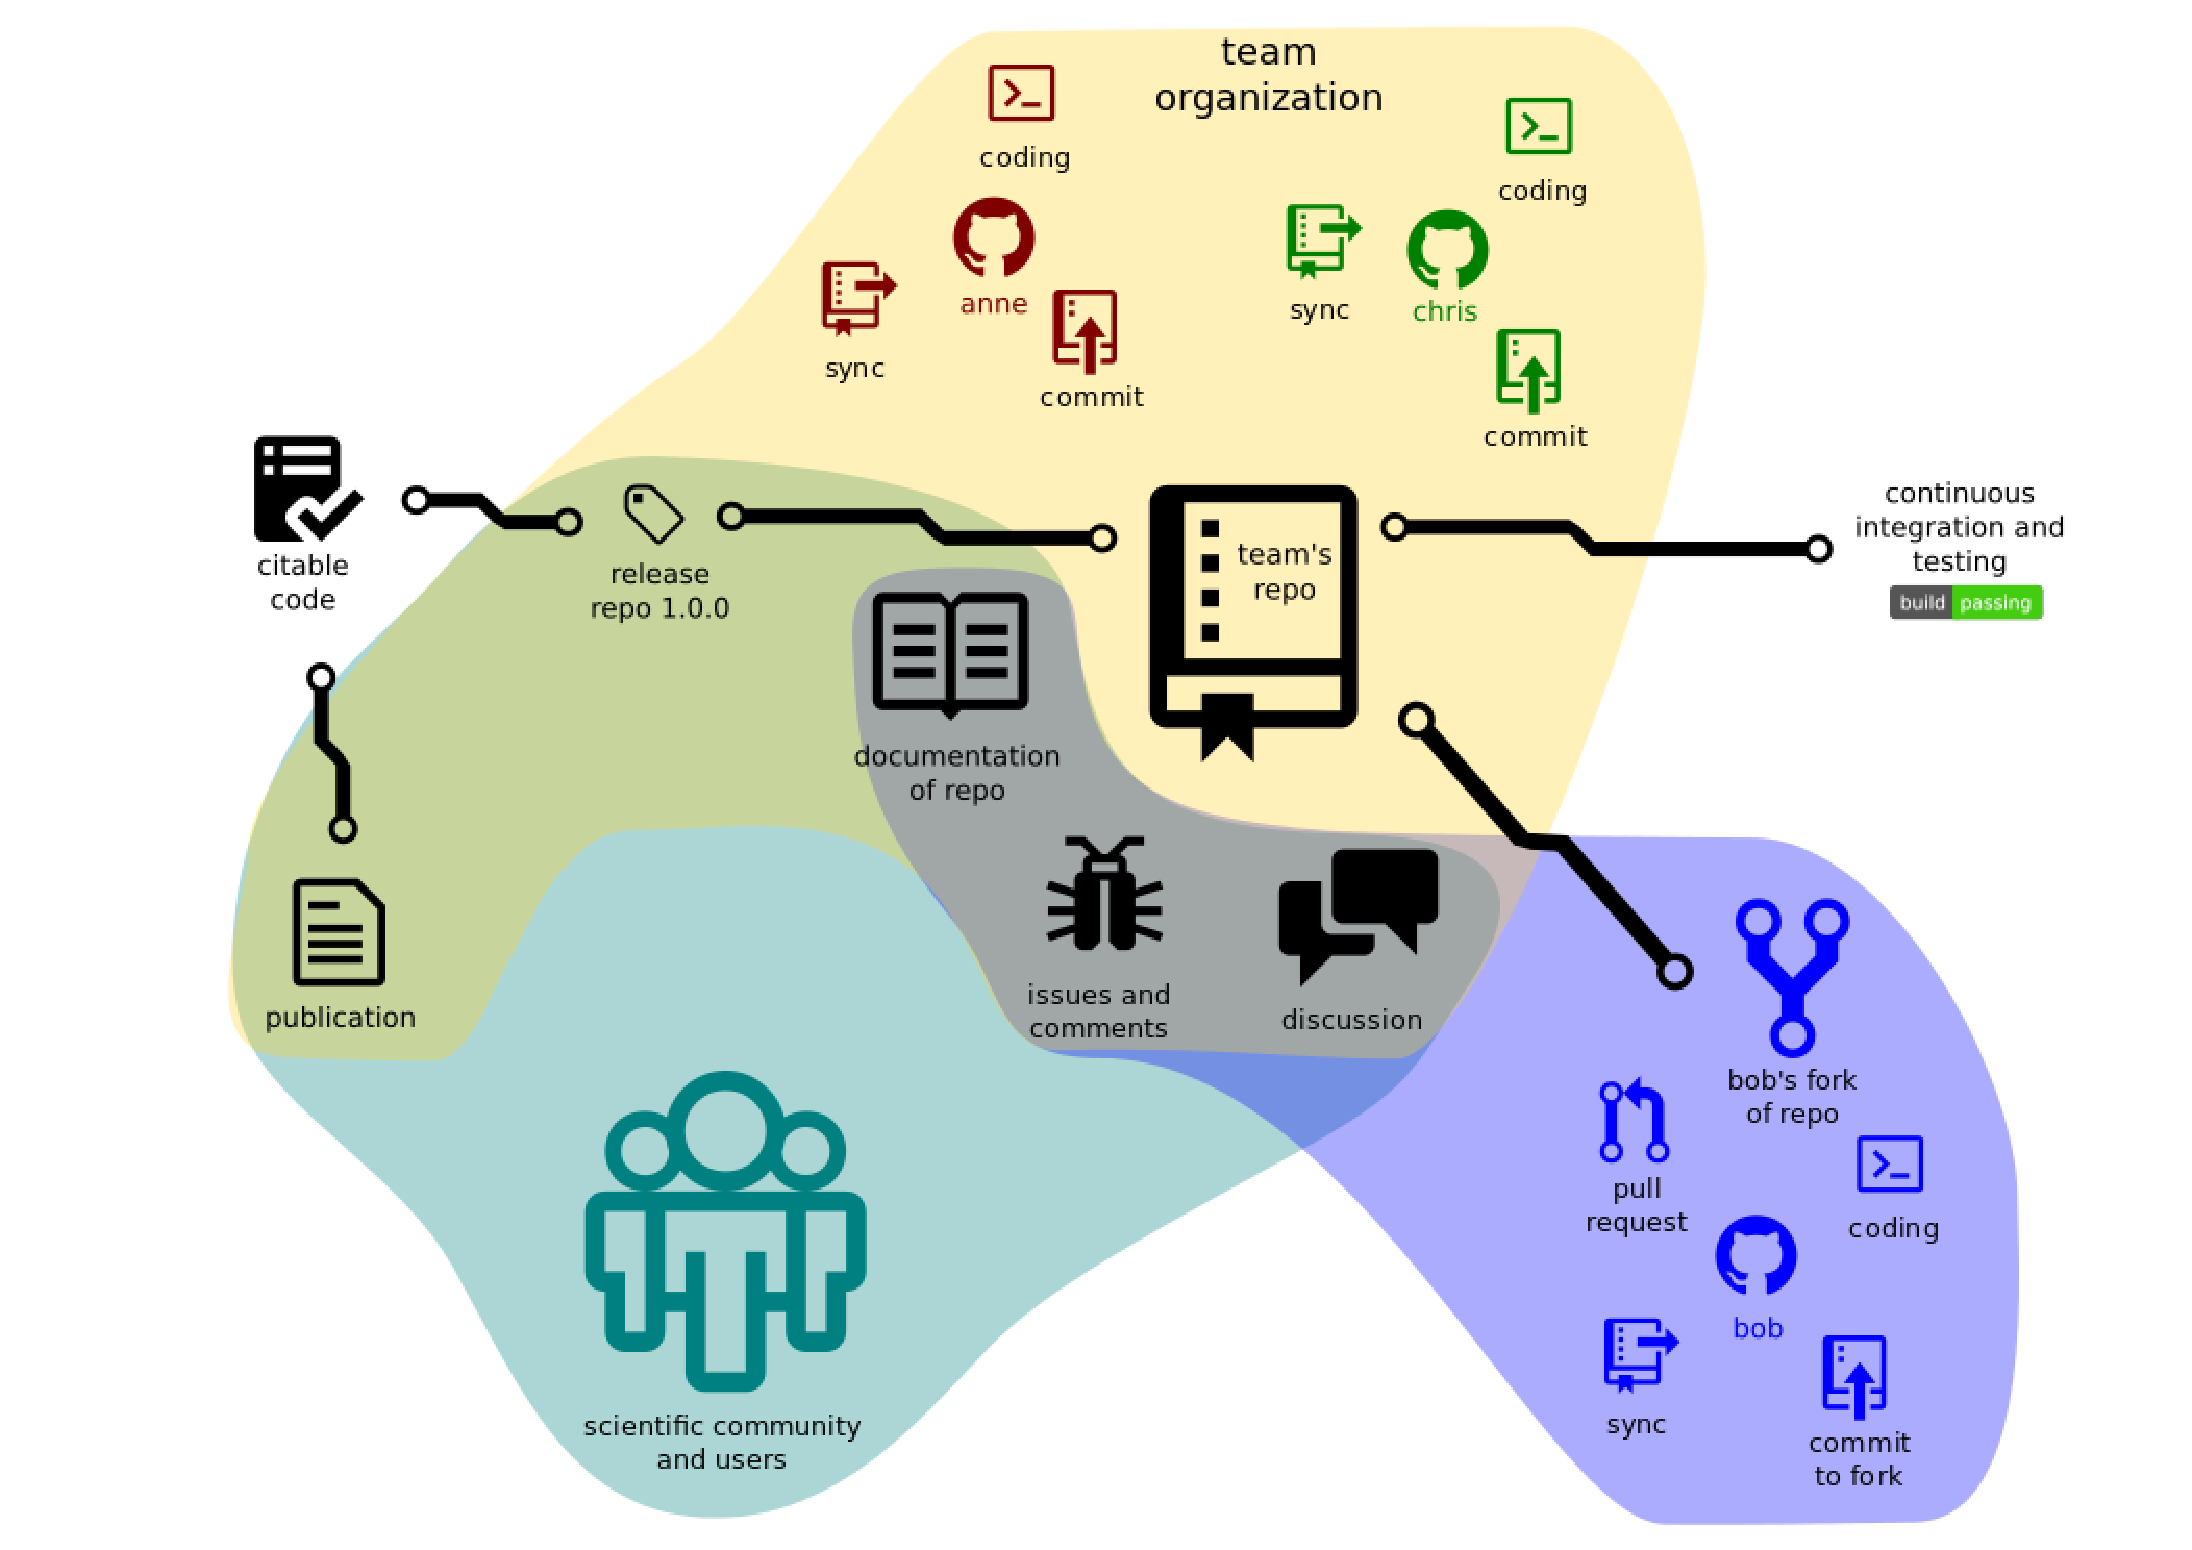
\includegraphics[width=\linewidth]{../figures/figure01_overview.pdf}
\caption{The structure of a GitHub-based project illustrating project
structure and interactions with the community.}
\end{figure}

\subsection*{Rule 2. Learn Git and embrace its
power}\label{rule-2.-learn-git-and-embrace-its-power}

The cornerstone of GitHub is the distributed version control system git.
Every change, from fixing a typo to a complete redesign of the software
is controlled by versions, so called revisions. While beginners may
consider the learning curve of Git steep, many introductory and detailed
tutorials are available. A revision can be considered as a
\emph{snapshot} (version) of a file system. Git is remarkably effective
in archiving the complete history of a project (all revisions) by,
amongst other things, storing only the differences among them. To create
a new revision, the set of changes introduced (e.g.~new, deleted or
modified files) are committed to the repository. Following the rule:
``commit often, as most as you can, perfection later'', one can keep
track of the development in small incremental changes. At any time it is
possible to go back to a previous version. In larger projects, multiple
users contribute to the same repository.

\subsection*{Rule 3. Use branches}\label{rule-3.-use-branches}

Concurrent development including commits to the same repository can be
organised using several common approaches. The most common way is to use
git \emph{branches} to separate different lines of development. Active
development is often performed on a development branch and stable
versions e.g.~those used for a software release, are kept in a master
branch. In practice, developers work on one or several features or
improvements. To keep commits of the different features logically
separated, distinct branches are typically used. Later, when development
is complete and none of the tests fail (see Rule 6) new features can be
merged back into the development line or master branch. During such a
development, the original branch might continuously be developed and
other features might be merged into the master branch. Nevertheless, one
can always pull the currently up-to date master branch into one fork,
always enabling to react or adapt to the changes in the code. In
projects involving more than one contributor, everyone wants to be sure
that the contributions of others increase the quality and move the
project forward. \emph{Forking} a repository and providing \emph{pull
requests} constitute an easy way for collaboration inside and over
organisations boundaries. A user that forks a repository creates a copy
under their GitHub account. Modifications like a branch with new
features or bug fixes can conveniently be provided to the forked
(upstream) repository by opening a pull request. Once it is opened for
review and discussion, it usually results in additional insights and in
an increased code quality. Once a pull request gets accepted, typically
it gets merged into the development branch.

\subsection*{Rule 4. Use tags and semantic version
numbering}\label{rule-4.-use-tags-and-semantic-version-numbering}

Tags offer the possibility to label versions during the development
process, tracking its progress. Version numbering should follow semantic
versioning in the form X.Y.Z, with X being the major, Y the minor and Z
the patch version of the release, including possible meta information,
as described in http://semver.org/. Correct labelling allows developers
and users to easily recover older versions, compare them, or simply use
them to reproduce results described in publications (see Rule 8). This
approach will also help defining a coherent software publication
strategy (see Rule 6).

\subsection*{Rule 5. The code must always be ready to use: continuously
integrate}\label{rule-5.-the-code-must-always-be-ready-to-use-continuously-integrate}

The first rule of software development is that the code needs to be
ready to use as soon as possible \cite{Leprevost:2014}, remain so during
development, and should be well-documented and tested. In 2005, Martin
Fowler defined the basic principles for continuous integration in
software development \cite{FowlerCI}. These principles have become the
main reference for best practices in continuous integration, providing
the framework needed to deploy software, and in some way also data.
Every repository, script, mathematical model, and function should
contain a set of self-automated tests. A source code may run, but that
does not mean it is doing the right thing. The simple use of those
self-automated tests is to detect possible bugs introduced by new
features, or changes in the code or dependencies, but also to detect
wrong results, the so called \emph{logic errors}, where the source code
produces a different result compared to what one intended it to do.
Then, continuous integration provides the way of automatically run all
of these tests in the repository by checking data and software
dependencies. Continuous integration can be done automatically on GitHub
(See Rule 6).

\subsection*{Rule 6: Automate for better code
quality}\label{rule-6-automate-for-better-code-quality}

GitHub offers different types of hooks that are executed after each push
to a repository, making easier to follow the basic principles of
continuous integration. The GitHub web hooks allows third-party
platforms to access and interact with a GitHub repository and thus to
automate post-processing tasks. Such tasks demonstrate to the community
that a project follows rigorous software engineering processes, often
associated with high quality development. It also shows that is
currently working and has documentation that reflects the current code.
We suggest that all these three tasks become part of your project.
Firstly, continuous integration can be achieved by \emph{Travis}
(https://travis-ci.org), a hosted continued integration platform that is
free for all open source projects. Travis builds and tests the source
code using a plethora of options such as different platforms and
interpreter versions. Furthermore it offers notifications which allow
your team and contributors to know if the new changes work, and prevent
the introduction of errors in the code, making the repo always ready to
use. Secondly, in addition to successful completion of the tests, one
can also demonstrate that they cover the existing code base
sufficiently. For this task, the integration of \emph{Codecov} is
recommended (https://codecov.io). Thirdly, one might consider to
automatically update the documentation upon code modification. This
implies that your projects provide comprehensive documentation so others
can understand, and contribute back to them. For Python or C/C++ code,
automatic documentation generation can be done using sphinx
(http://sphinx-doc.org/) and subsequently integrated into GitHub using
``Read the Docs'' (https://readthedocs.org/). All of these platforms
will create reports and badges (also called shields) for the projects
that can be included on your GitHub page, thereby making your projects
easily identifiable as high quality and well-maintained.

\subsection*{Rule 7. Use and maintain your GitHub issue
trackers}\label{rule-7.-use-and-maintain-your-github-issue-trackers}

GitHub \emph{issues} are a great way to keep track of bugs, tasks, and
enhancements. Classical issue trackers are primarily intended to be used
as bug trackers. In contrast, GitHub issues follow a different
philosophy: each tracker has its own section in every repository, and
can be used to trace bugs, new ideas, and enhancements, by using a
powerful but optional tagging system for each issue. Its main focus is
put in promoting collaboration, providing context by using
cross-references, and an excellent text formatting for each issue: (i) a
title and description, (ii) colour-coded labels help to categorise and
filter issues, (iii) milestones act as a container for issues,(iv) one
assignee responsible for working on the issue, and (v) comments that
allow anyone with access to the repository to provide feedback. Another
aspect is its simplicity. For instance, it does not require to fill
lengthy forms including every piece of information that might be
valuable to reproduce the bug. It only requires to give the title and
provide some optional text. If the developer needs more information,
they can simply request it in a comment. GitHub issues are then more
dynamic and pose a lower barrier for users to report bugs and request
features. A well-organised and tagged issue tracker will help upcoming
contributors and users to understand a project more deeply.

\subsection*{Rule 8. Make your code easily citable, and cite source
code!}\label{rule-8.-make-your-code-easily-citable-and-cite-source-code}

In research, it is a good practice to ensure permanent and unambiguous
identifiers for citable items like articles, datasets, or biological
entities such as proteins, genes and metabolites, among others. Digital
Object Identifiers (DOIs) have been used for many years as unique and
unambiguous identifiers for enabling the citation of scientific
publications. More recently, a trend has started to produce DOIs for
other types of scientific outputs such as datasets \cite{Vizcaino:2014}
or training materials (for example \cite{Ahmadia_2015_27353}). The main
motivation behind this is to give scientists a better credit for their
work \cite{NatBiotechEditorial:2009}, enabling at the same time a better
way to cite and track it. A common issue with software is that it
normally evolves at a different speed than what is published in the
scientific literature. In fact, it is common to find software having
novel features and functionalities that were not described in the
original publication. GitHub now enables the use of DOIs to cite the
code deposited, using the data archiving tool Zenodo
(https://zenodo.org/). The procedure is simple (see
https://guides.GitHub.com/activities/citable-code/) and, by default,
Zenodo takes an archive of a repository each time a new release is
created in GitHub. However, before Zenodo can issue a DOI, metadata
needs to be provided about the archived repository. Once the DOI has
been assigned, apart from using it in your CV, you can add it to
literature information resources such as Europe PubMed Central
\cite{EuropePMCConsortium:2015}. As already mentioned in the
introduction, reproducibility of scientific claims should be enabled by
providing openly the software, the datasets and the process leading to
interpretable results that are used in a particular study. One should
always highlight as much as possible in publications that the code is
freely available in, for example, GitHub, together with any other
relevant piece of information that may have been deposited. In our
experience, this openness substantially increases your chances of
getting the paper accepted for publication. On one hand, journal editors
and reviewers have the opportunity to reproduce your findings during the
manuscript review process, increasing the confidence of your results. On
the other hand, once the paper is published, your work can be reproduced
by any member of the scientific community, which can increase citations
and foster opportunities for further discussion and collaboration. Also
one must have in mind that the availability of a public repository with
the source code does not make the software open source \emph{per se}, as
it needs to have an appropriate license
(http://opensource.org/licenses/).

\subsection*{Rule 9. Promote your projects in the scientific community -
create a web page and
more}\label{rule-9.-promote-your-projects-in-the-scientific-community---create-a-web-page-and-more}

Additional steps can be done to boost the visibility of a organisation.
For example, GitHub \emph{Pages} are simple landing webpages that GitHub
hosts for free without the need for a server or database. GitHub users
can create and host blog websites, help pages, manuals, tutorials and
websites related to specific projects. \emph{Pages} comes with a
powerful static site generator called Jekyll (https://jekyllrb.com) that
can be integrated with other platforms such as Bootstrap
(http://getbootstrap.com/) or Disqus (https://disqus.com/), to support
and moderate comments. In addition, GitHub also provides mechanisms for
real-time communication called Gitter (http://gitter.im). Gitter is a
GitHub-based chat tool (in limited beta at the time of writing) which
enables developers and users to share aspects of their work. Gitter
inherits the shape of the social groups operating around GitHub
repositories, organisations, and issues. It relies on the identity
within GitHub, creating IRC (Internet Relay Chat)-like chat rooms for
public and private repositories. From within a Gitter chat, members can
reference issues, comments, or pull-requests. A different service is
Gist (https://gist.github.com), which represents a unique way to share
\emph{code snippets}, single files, parts of files, or full
applications. Gist can be generated in two different ways: public
\emph{gists}, that can be browsed and searched, and secret gists that
are not provided through \emph{Discover}
(https://gist.github.com/discover). One of the main features of Gist is
the possibility to embed code snippets in other applications, enabling
users to embed gists in any text field that supports JavaScript.

\subsection*{Rule 10. Check periodically existing open source
projects}\label{rule-10.-check-periodically-existing-open-source-projects}

One of the main tasks of scientists is to actively follow the
developments in their field. Analogously, scientific programmers need to
revise publicly available (e.g.~open source) projects and code that can
be interesting for their research. Therefore, you should try to learn as
much as possible from your peers and keep up-to-date with all the
developments of relevant projects. GitHub enables this functionality by
\emph{following} other GitHub users (also mentioned in Rule 1) or
\emph{watching} the activity of projects, which is a common feature in
many social media platforms. Take advantage of it as much as possible!

\subsection*{Conclusions}\label{conclusions}

If you are interested and have not used GitHub so far, we recommend you
to get started as soon as possible. As in any other topic, a learning
curve is required for beginners. However, we anticipate the reward will
be worth your effort.

\subsection*{Disclaimer}\label{disclaimer}

The authors have no affiliation with GitHub, nor any commercial entity
mentioned in this article. The views described here reflect our own
without any input from any third party organisation.

\nolinenumbers

\bibliography{refs.bib} 

\end{document}

